\subsection{Modelo}

Recordemos que el objetivo principal del acceso a los datos, es obtener conocimiento. Hay que tener en 
cuenta que los datos por si solos, no tienen ningun valor, ya que carecen de sentido, una vez integrados en un contexto,
nos aportara informacion, y procesando y analizando esta informacion, se obtendra el conocimiento.\\
    
\begin{figure}[ht]
    \centering 
    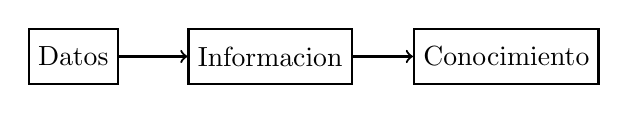
\begin{tikzpicture}[thick]
        \node[draw,rectangle,minimum size=20] (a) {Datos};
         \node[draw,rectangle,minimum size=20,right of= a, node distance=2.5cm] (b) {Informacion};
         \node[draw,rectangle,minimum size=20,right of=b, node distance=3cm] (c) {Conocimiento};
         \draw[->] (a) to (b);
        \draw[->] (b) to (c);
     
      \end{tikzpicture}
      \caption{Diagrama. De datos a conocimiento}
    \end{figure}
 
Para poder obtener este conocimiento de los datos, es necesario que el usuario interprete correctamente los datos, no
simplemente que significan los valores y las unidades, sino que representan. Por lo
que el usuario debe contar con conocimientos en la materia o realizar una tarea de investigacion, que le permita 
entender los datos extraidos. 

Para poder construir un sistema que haga los datos accesibles, es imprescindible disenar un modelo  para concretar la 
informacion que se desea obtener. El diseno de un sistema permitira que a partir de unos valores dados, proporcione unos resultados.
Para ello sera necesario tener un conocimiento solido del conjunto de datos que se necesita, los valores,
sus unidades y como se relacionan entre si.

Asi pues, para que el usuario pueda obtener la informacion de una manera directa, requiere de conocimientos tanto 
de programacion como especificos de la materia y los recursos para crear una infraestructura que le permita implementar 
una representacion de los datos que le sea util.


\subsubsection{How to solve it} 
Estudiar el objetivo buscado y recurrar a la ayuda de expertos si fuera necesario para adquirir los conocimientos necesarios
sobre la materia. Disenar un modelo que proporcione la informacion que buscamos. 

\subsubsection{How we solve it. Aire Guru} 
Aire Guru tiene como objetivo aumentar el concienciamiento del nivel de polucion que nos rodea, para ello utiliza una medida llamada
el indice de calidad del aire (AQI) concretamente el indice de calidad del aire europeo (EAQI).


\newpage
\begin{figure}[ht]
    \centering
    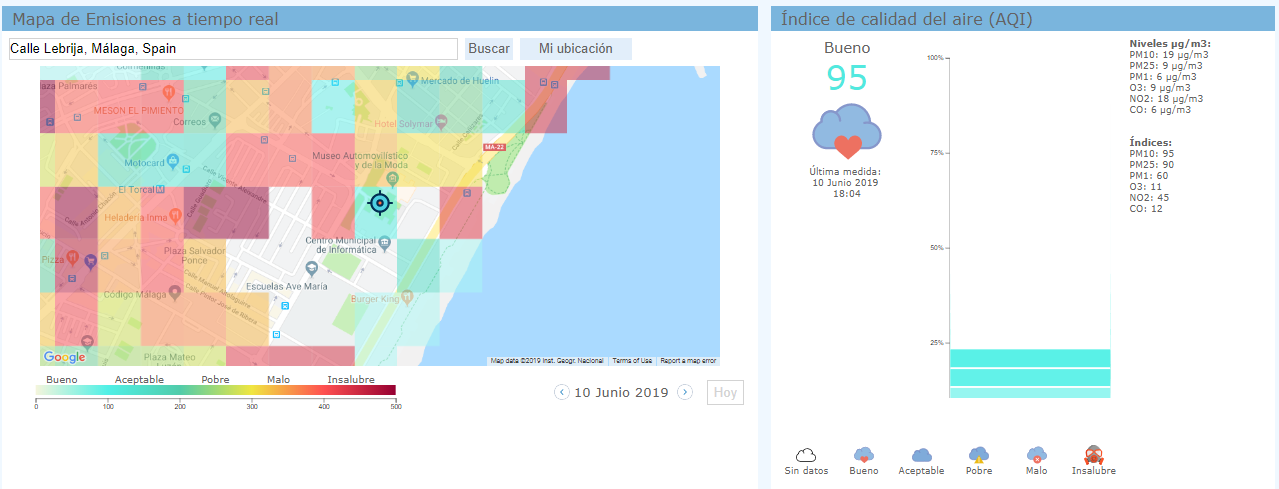
\includegraphics[width=10cm]{mapAireGuru}
    \caption{Aire Guru. Landing page. Top section}
\end{figure}

Aire Guru se comprende de distintas secciones. Mediante la seleccion de un punto en el mapa, nos
mostrara informacion detallada de este punto. A continuacion, cuenta con una seccion que filtrara la informacion acorde a las preferencias del usuario
y para concluir, muestra el historial de los contaminantes desde 2018 y el historial de la polucion al que el usuario ha estado
expuesto.

Es de preveer que el usuario estara interesado en el nivel de polucion al que esta expuesto a tiempo real, por ello, para usuarios
que esten identificados y accedan a compartir su ubicacion, Aire Guru mostrara directeramente la polucion en el punto en el 
que se encuentra.

El workflow de las distintas secciones de Aire Guru esta detalladamente estudiada. Como vemos en la Figura X. Aire Guru. Landing page. Top section, el punto de partida es la localizacion que nos interesa,
a continuacion se muestra la informacion general de este punto, el AQI general, despues el AQI de cada uno de los contaminantes que componen el 
AQI general y por ultimo los valores numericos de cada uno de los contaminantes. Como vemos vamos de menos a mas detalle.

\elsparagraph{Evaluation}  

\begin{itemize}
\done La informacion queda centrada en un objetivo, informar al usuario el nivel de polucion que le rodea a tiempo real
y en el pasado
\done La informacion sigue un hilo logico. History telling
\done El usuario encuentra la informacion mas importante con el minimo esfuerzo, simplemente con abrir la pagina
\end{itemize}

\newpage